\chapter{Component Information}
This section details the definition, background information, and purpose for each component.
\section{Propulsion}
The motors and propellers work together to achieve a desired thrust. Many factors play into the amount of thrust, speed, and noise of the motor-propeller assembly. 

\subsection{Motor}
Brushless DC motors (BLDC) are the common motors used for quadcopter drones. 
Motor selection depends on required thrust, thrust depends on the total weight of the frame size. Generally, the thrust to weight ratio (TWR) in Equation \ref{eq1} is used to select a motor.
\begin{equation} \label{eq1}
TWR = \frac{T}{W}
\end{equation}
Where \textit{T} is the thrust and \textit{W} is weight, both in Newtons or pounds.

For the drone to be able to take off, a TWR $>$ 1 is required. Once the drone flies at an inclination, the thrust is split into x and y components. This means that the y-component of the thrust can drop. So for a TWR $ \geq $ 1.3 would be required for a maximum inclination angle of 40. In general, a TWR $ \geq $ 2.0 should be used at a minimum, so with 4 motors, each motor must provide a thrust equal to the mass divided by 4. (Cite quadcopter paper)

The constant velocity of a motor ($K_v$) is defined as the number of RPMs a motor will turn when 1V is applied with no load. 

\subsection{Propeller}
There are a couple of specifications that determine the performance of the propeller. Pitch, size, the number of blades; propeller material, and propeller weight \cite{droneomega}

The pitch of a propeller is defined as the distance the propeller would move in one revolution if it were moving through a soft solid. The higher the pitch, the faster the drone will fly. This is analogous to a screw; the pitch is measured the same way. The pitch must not be too flat or too steep as this will result in no lift being generated. 

\begin{figure}[!htb]
	\graphicspath{ {Images/} }
	\centering
	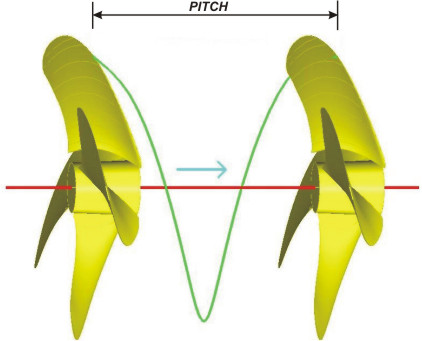
\includegraphics[width=0.6\textwidth,scale=0.8]{propeller.jpg}
	\caption{Propeller pitch }
	\label{fig:propeller}
\end{figure}

The length of the propeller from tip-to-tip is the defined as the length. Longer propellers generate more thrust for the same speed but require more torque from the motor. 

Number of blades - what effect does adding blades have?

Propeller material and weight - how does this affect performance? Noise? Would a smoother material be quieter? is noise caused by surface roughness or vibrations in the propeller along it's length?

\section{Chassis}
The chassis includes the internal frame, the arms, and the landing feet. 

Detail what characteristics each part of the chassis should have.

\hl{It might be helpful to develop a finite element model (FEM) of the top and bottom plates with the arms attached to determine optimal plate material and thickness.}

NOTE: Make a table comparing manufacturing techniques; 3D printing, injection moulding.

Look for other manufacturing techniques for landing gears and other common parts.

\subsection{Frame Design}
The size of the drone will depend on several factors. The size of the propellers, battery pack, and electronics. 
The frame of the drone will be constructed of 3D printed nylon parts because this allows for modularity and easy replacement of parts in the event of a failure. 
The top and bottom plates will compress the arms to hold them in place,  these plates will need to be stiff? (check) The arms need to be held in tight between the plates, we should consider adding some vibration damping between the plates to reduce transfer to the electrical components.

Why should their be a power and reset on the outside? Just quickly explain why.


\subsection{Arms}
Define what the arms are.

The arms must be long enough so that the frame does not hinder the function of the propulsion system. The arms must also be thin enough to ensure thrust is not reduced during operation. (not sure if this would make a big difference, could test in motor testing rig by placing different sized arms behind propeller and measure the drop in performance)

\subsection{Landing Feet}
Define what the landing feet are.

The feet could be placed in two different locations. Either beneath the motors at the end of the arms or near the body at the beginning of the arms. An analysis of the best location should be conducted with consideration placed on durability of body on hard landings and the landing platform. (Compare the two placements, pros and cons)

\section{Electronics}

\subsection{Computer and Carrier Board}
Define what the computer and carrier board do. 

What functions do they serve on the drone?

\subsection{Flight Controller}
Define what the flight controller does.

\subsection{Electronic Speed Controller}
The electronic speed controller (ESC) send pulse width modulation (PWM) signals to the motors to control the speed \hl{(source)}

\subsection{GNSS/Compass}
Define what the GNSS/Compass does.

\subsection{Optical Components}
Define what role the optical components do; image recognition, finding landmarks, determining the distance to objects, etc. 

The optical components are the cameras and the range finder.

\subsection{Power}

This includes the batteries and battery pack design. \\

Two types of lithium batteries are being considered, the lithium ion and lithium polymer batteries. Both have advantages and disadvantages compared to one another. \\

The major difference between lithium ion and lithium polymer batteries is the type of electrolyte used. LiPo batteries use a micro porous electrolyte as opposed to a liquid electrolyte and a porous separator. They also contain laminated sheets which eliminates the need for compression. Since the LiPo batteries don’t need compression, they can be made into other shapes, such as a “pouch”. They offer a slightly higher specific energy, but the manufacturing cost can be higher than traditional cylindrical batteries. Other than that, the two batteries are essentially the same. They both use the same cathode and anode material and have the same amount of electrolyte. \\

Lithium ion batteries vary depending on the type of material used as the cathode. \hl{(Elaborate on this, could influence which batteries will be used)} reference\\



\subsection{Power Management}
The power management system consists of the power distribution board... Is there more?



What does the power distribution board do?

\subsection{Modular Payloads}
A feature of the Spiri is that it can accommodate different payloads mounted on it's underside. (should include picture here) A \textbf{payload} is defined as an additional component added to the drone to serve a specific function.
